\subsection{Prediction Under New Student Wording (RQ2)}
\label{sec:cue-results}

When students express themselves differently, the original model defaults still
help predict whether tutors give answers or invite reasoning. For acknowledgement,
the extra benefit of knowing each model's response to student cues is lost.
This benefit remains positive when we collect new replies using the original
wording during the same period. The contrast weakens an explanation based only on a general loss of predictive
value over time. Figure~\ref{fig:expression-transfer}
shows the estimates and uncertainty; Appendix Table~\ref{tab:cue-primary}
gives all six tests and Appendix~\ref{app:cue-transfer} the paired contrasts.

\begin{figure}[t]
\centering
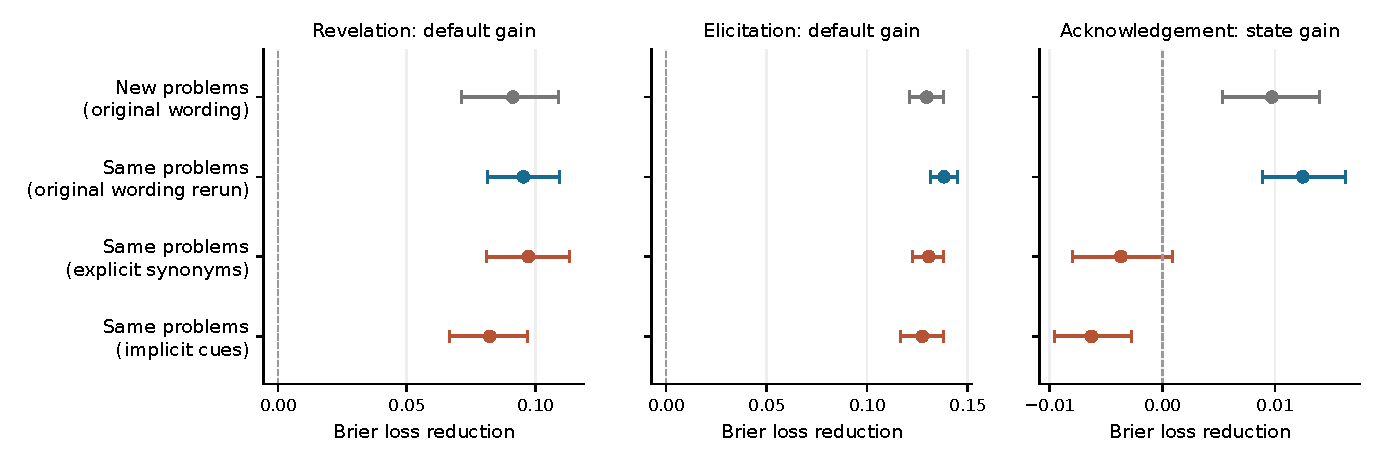
\includegraphics[width=\linewidth]{figures/expression_transfer.pdf}
\caption{Transfer depends on what is changed. The initial test uses
new problems with the original wording. The three follow-up conditions use
those same 32 problems and the earlier predictions. Default gains for giving answers and
inviting reasoning remain positive, while the state gain for acknowledgement
is no longer positive under new wording. Bars are source bootstrap 95\%
intervals conditional on frozen fits, not four independent replications or
simultaneous intervals. Horizontal scales differ by panel.}
\label{fig:expression-transfer}
\end{figure}

The acknowledgement gains have the same sign pattern when each annotator's labels
are used separately and when each generating model is left out, although some
intervals include zero. These checks reuse the same responses. The result
concerns prediction: models still acknowledge feeling or difficulty at different
rates for contrasting student cues. It does not mean that models stop responding to
student cues. The implicit condition also changes more than affect wording.

\paragraph{Alternative explanations.}
Losing an advantage over a baseline does not always mean making larger errors.
Under explicit synonyms, the cue-based predictor's own loss improves slightly,
yet it no longer outperforms the baseline. Under implicit cues, its own loss
also worsens. Further checks show that a common change in acknowledgement
frequency cannot explain the contrast, and the tested logistic recalibrations
do not restore a positive gain. These follow-up analyses narrow the explanations
without identifying a unique mechanism
(Appendices~\ref{app:cue-diagnosis}--\ref{app:cue-calibration}).

In the additional classmate control, changing a classmate's quoted feelings changes
acknowledgement rates even though the current student remains calm. Selected
examples show this can happen when the model correctly distinguishes the two
students' feelings. The contrast alone therefore does not establish confusion
about whose feelings are being expressed (Appendix~\ref{app:cue-transfer}).
